\documentclass[fleqn]{article}
\usepackage{amsmath, amssymb, esdiff}
\usepackage{gensymb}
\usepackage{commath}
\usepackage{tikz, pgfplots}
\usetikzlibrary{calc}
\usepackage{graphicx}
\usepackage{datetime}
\usepackage{ulem}
\usepackage{xcolor}
\usepackage{enumerate}
\setcounter{secnumdepth}{4}

\newcommand\numberthis{\addtocounter{equation}{1}\tag{\theequation}}

\newcommand{\AxisRotator}[1][rotate=0]{%
	\tikz [x=0.25cm,y=0.60cm,line width=.2ex,-stealth,#1] \draw (0,0) arc (-150:150:1 and 1);%
}

%opening
\title{Lecture 6}
\author{Aakash Jog}
\date{\formatdate{13}{11}{2014}}

\begin{document}

\maketitle
%\setlength{\mathindent}{0pt}

\tableofcontents

\newpage
\section{Circular Motion}

\subsection{Time Period}

Time period is defined as the time required to complete a full circle.
\begin{align*}
	T &\doteq \dfrac{2 \pi}{\omega}\\
	f \doteq \dfrac{1}{T} &= \dfrac{\omega}{2 \pi}
\end{align*}

\subsection{Angular Velocity}

\begin{align*}
	\overrightarrow{v} &= \overrightarrow{\omega} \times \overrightarrow{r}
\end{align*}

\subsection{Examples}

\subsubsection{Example 1}

If there is no friction, \\
%\begin{figure}[ht!]
%	\includegraphics[width=4in, angle=-90]{IMG_3940.JPG}
%\end{figure}
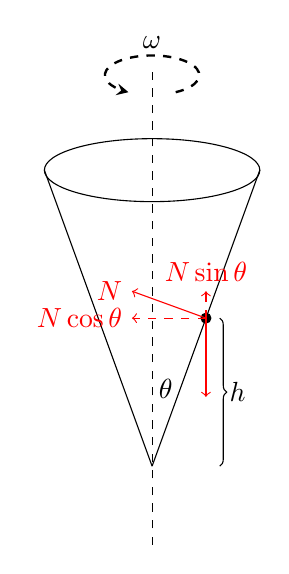
\begin{tikzpicture}
	\draw (0,0) -- (70:4);	
	\draw (0,0) -- (110:4);
	\draw (0, {4*cos{20}}) circle [x radius = {4*sin{20}}, y radius = 0.4];
	\draw [dashed] (-90:1) -- (90:5) node {\AxisRotator[rotate=90] };
	\node at ({70+((90-70)/2)}:1) {$\theta$};
	\node [above, yshift=5] at (90:5) {$\omega$};
	
	\fill (70:2) circle [radius=2pt];
	
	\draw [red, ->](70:2) -- ++(-90:1);
	
	\draw [red, ->](70:2) -- ++(160:1) node [left] {$N$};
	\draw [red, ->, dashed](70:2) -- ++(90:{sin 20}) node [above] {$N \sin \theta$};
	\draw [red, ->, dashed](70:2) -- ++(180:{cos 20}) node [left] {$N \cos \theta$};
	
	\draw [decorate, decoration={brace}, xshift=5] (70:2) -- ++(-90:{2*cos 20}) node [midway, right] {$h$};
\end{tikzpicture}
\begin{align*}
	N \sin \theta_0 &= m g \\
	N \cos \theta_0 &= m \omega^2 R \\
	\therefore \cot \theta_0 &= \dfrac{\omega^2 h \tan \theta_0}{g}\\
	\therefore T_0 &= 2 \pi \sqrt{\dfrac{h}{g}} \tan \theta_0
\end{align*}

If friction is directed upwards,\\
%\begin{figure}[ht!]
%	\includegraphics[width=4in, angle=-90]{IMG_3941.JPG}
%\end{figure}
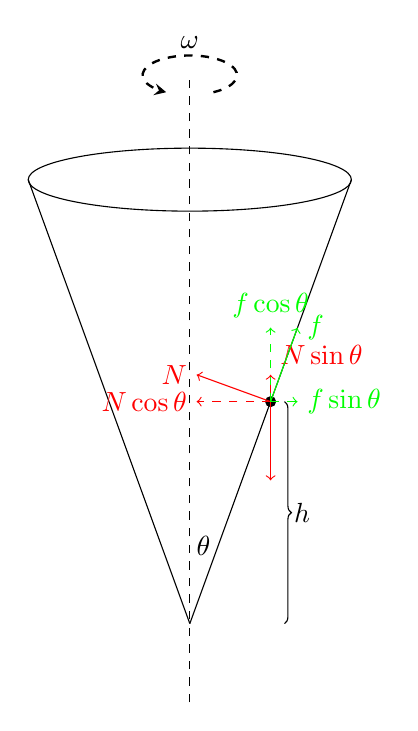
\begin{tikzpicture}
	\draw (0,0) -- (70:6);	
	\draw (0,0) -- (110:6);
	\draw (0, {6*cos{20}}) circle [x radius = {6*sin{20}}, y radius = 0.4];
	\draw [dashed] (-90:1) -- (90:7) node {\AxisRotator[rotate=90] };
	\node at ({70+((90-70)/2)}:1) {$\theta$};
	\node [above, yshift=5] at (90:7) {$\omega$};

	\fill (70:3) circle [radius=2pt];

	\draw [red, ->](70:3) -- ++(-90:1);

	\draw [red, ->](70:3) -- ++(160:1) node [left] {$N$};
	\draw [red, ->](70:3) -- ++(90:{sin 20}) node [above right] {$N \sin \theta$};
	\draw [red, ->, dashed](70:3) -- ++(180:{cos 20}) node [left] {$N \cos \theta$};

	\draw [decorate, decoration={brace}, xshift=5] (70:3) -- ++(-90:{3*cos 20}) node [midway, right] {$h$};
	
	\draw [green, ->](70:3) -- ++(70:1) node [right] {$f$};
	\draw [green, dashed, ->](70:3) -- ++(0:{sin 20}) node [right] {$f \sin \theta$};
	\draw [green, dashed, ->](70:3) -- ++(90:{cos 20}) node [above] {$f \cos \theta$};
\end{tikzpicture}
\begin{align*}
	f \cos \theta_0 + N \sin \theta_0 &= m g \\
	N \cos \theta_0 - f \sin \theta_0 &= m \omega^2 R \\
	&= m \omega^2 (h \tan \theta_0) \\
	\therefore T_{\text{max}} &= T_0 \sqrt{\dfrac{\cos \theta_0}{\sin \theta_0} \cdot \dfrac{\mu_s \cos \theta_0 + \sin \theta_0}{\cos \theta_0 - \mu \sin \theta_0}} 
\end{align*}

If friction is directed downwards,
\begin{align*}
	- f \cos \theta_0 + N \sin \theta_0 &= m g \\
	N \cos \theta_0 + f \sin \theta_0 &= m \omega^2 R \\
	&= m \omega^2 (h \tan \theta_0) \\
	\therefore T_{\text{min}} &= T_0 \sqrt{\dfrac{\cos \theta_0}{\sin \theta_0} \cdot \dfrac{- \mu_s \cos \theta_0 + \sin \theta_0}{\cos \theta_0 + \mu \sin \theta_0}} 
\end{align*}

\subsubsection{Example 2}

\begin{tikzpicture}
	\draw (0,0) circle [radius = 4];
	\draw [dashed] (0,0) -- ++(125:4) node [midway, fill=white] {$R$};
	
	\fill (0,0) circle [radius = 1pt];
	
	\draw (0,3.75) circle [radius = 0.25];
	\draw [->] (0,3.75) -- ++(-90:1) node [below] {$mg$};
	\draw [->] (0,3.75) -- ++(-90:0.5) node [right] {$N$};
	
	\draw (3.75,0) circle [radius = 0.25];
	\draw [->] (3.75,0) -- ++(-90:1) node [below] {$mg$};
	\draw [->] (3.75,0) -- ++(180:0.5) node [below] {$N$};
	
	\draw (0,-3.75) circle [radius = 0.25];
	\draw [->] (0,-3.75) -- ++(-90:1) node [below] {$mg$};
	\draw [->] (0,-3.75) -- ++(90:0.5) node [right] {$N$};
	
	\draw (35:3.75) circle [radius = 0.25];
	\draw [dashed] (0,0) -- ++(35:3.75);
	\node at ({35/2}:1) {$\theta$};
	\draw [dashed] (0,0) -- ++(0:3.75);
	\draw [red, ->] (35:3.75) -- ++(-90:1) node [below] {$mg$};
%	\draw [green, ->] (35:3.75) -- ++(215:!sin 35!) node [left] {$mg \sin \theta$};
%	\draw [green, ->] (35:3.75) -- ++(305:!\sin 35!) node [left] {$mg \cos \theta$};
	\draw [red, ->] (35:3.75) -- ++(215:0.5) node [above left] {$N$};
\end{tikzpicture}

At the topmost point, if the ball just completes the circular motion
\begin{align*}
	m g &= m \dfrac{v^2}{R} \\
	\therefore v &= \sqrt{g R}
\end{align*}

At a point at angle $\theta$ from the horizontal,
\begin{align*}
	(- N - m g \sin \theta) \hat{r} - m g \cos \theta \hat{\theta} &= - m R (\dot{\theta})^2 + m R \ddot{\theta} \hat{\theta} \\
	\therefore - N - m g \sin \theta &= - m R (\dot{\theta})^2 \\
	\therefore - m g \cos \theta &= m R \ddot{\theta}
\end{align*}

\subsubsection{Example 3}
\begin{tikzpicture}
	\draw (0,0) circle [radius = 4];
	\draw [dashed] (0,0) -- ++(125:4) node [midway, fill=white] {$R$};

	\fill (0,0) circle [radius = 1pt];

	\draw (35:3.75) circle [radius = 0.25];
	\draw [dashed] (0,0) -- ++(35:3.75);
	\node at ({35/2}:1) {$\theta$};
	\draw [dashed] (0,0) -- ++(0:4);
	
	\draw [red, ->] (35:3.75) -- ++(215:0.5) node [above left] {$N$};
	
	\draw [red, ->] (35:3.75) -- ++(305:0.5) node [right] {$f = \mu N$};
	
	\draw [green, ->] (35:3.75) -- ++(35:0.5) node [right] {$\hat{r}$};
	
	\draw [green, ->] (35:3.75) -- ++(125:0.5) node [left] {$\hat{\theta}$};
\end{tikzpicture}

\begin{align*}
	- N \hat{r} - \mu N \hat{\theta} &= - m R (\dot{\theta})^2 \hat{r} + m R \ddot{\theta} \hat{\theta}\\
	\mu m R (\dot{\theta})^2 &= - m R \ddot{\theta}\\
	\therefore \mu \omega^2 &= - \dot{\omega} \\
	&= - \dod{\omega}{t}\\
	\therefore \int \mu \dif t &= \int - \dfrac{\dif \omega}{\omega^2}
	\therefore \mu t + c = \dfrac{1}{\omega}
\end{align*}
At $t = 0$, $\omega = \omega_0$
\begin{align*}
	\therefore c &= \dfrac{1}{\omega_0} \\
	\therefore \mu t + \dfrac{1}{\omega_0} &= \dfrac{1}{\omega} \\
	\therefore \dod{\theta}{t} = \omega(t) &= \dfrac{\omega_0}{\mu \omega_0 t + 1} \\
	\therefore \theta(t) &= \dfrac{1}{\mu} \ln \left(\mu \omega_0 t + 1\right) + c_1
\end{align*}

\subsubsection{Example 4}
If,
\begin{align*}
	r &= 4\\
	\dot{r} = \ddot{r} &= 0\\
	\theta &= \dfrac{\pi}{2} t \\
	\dot{\theta} &= \dfrac{\pi}{2} \\
	\ddot{\theta} &= 0
\end{align*}
Find $\overrightarrow{v}$

\paragraph*{Solution\\}
\begin{align*}
\overrightarrow{r} &= r \hat{r} \\
\overrightarrow{v} = \dot{\overrightarrow{r}} &= \dot{r} \hat{r} + r \dot{\theta} \hat{\theta} \\
\overrightarrow{a} = \ddot{\overrightarrow{r}} &= \left(\ddot{r} - r(\dot{\theta})^2\right) \hat{r} + \left(2 \dot{r} \dot{\theta} + r \ddot{\theta}\right) \hat{\theta}
\end{align*}
Therefore,
\begin{align*}
	\overrightarrow{r} &= 4 \hat{r} \\
	\overrightarrow{v} &= 4 \dfrac{\pi}{2} \hat{\theta} = 2 \pi \hat{\theta}
\end{align*}
Therefore, 
\begin{align*}
	\overrightarrow{r} &= 4 \cos \left(\dfrac{\pi}{2} t \right) \hat{x} + 4 \sin \left(\dfrac{\pi}{2} t \right) \hat{y} \\
	\overrightarrow{v} &= - \dfrac{\pi}{2} \cdot 4 \sin \left(\dfrac{\pi}{2} t \right) \hat{x} + \dfrac{\pi}{2} \cdot 4 \cos \left(\dfrac{\pi}{2} t \right) \hat{y} \\
	&= - 2 \pi \sin \left(\dfrac{\pi}{2} t \right) \hat{x} + 2 \pi \cos \left(\dfrac{\pi}{2} t \right) \hat{y}
\end{align*}

\subsubsection{Example 5}

If,
\begin{align*}
	r &= v_0 t 
	&\dot{r} &= v_0
	&\ddot{r} &= 0 \\
	\theta &= \omega_0 t
	&\dot{\theta} &= \omega_0
	&\ddot{\theta} &= 0
\end{align*}

\paragraph*{Solution\\}

\begin{align*}
\overrightarrow{r} &= r \hat{r} \\
\overrightarrow{v} = \dot{\overrightarrow{r}} &= \dot{r} \hat{r} + r \dot{\theta} \hat{\theta} \\
\overrightarrow{a} = \ddot{\overrightarrow{r}} &= \left(\ddot{r} - r(\dot{\theta})^2\right) \hat{r} + \left(2 \dot{r} \dot{\theta} + r \ddot{\theta}\right) \hat{\theta}
\end{align*}
Therefore,
\begin{align*}
	\overrightarrow{r} &= v_0 t \hat{r} \\
	\overrightarrow{v} &= v_0 \hat{r} + v_0 t \omega_0 \hat{\theta} \\
	\overrightarrow{a} &= - v_0 t \omega_0^2 \hat{r} + 2 v_0 \omega_0 \hat{\theta}
\end{align*}
Therefore, 
\begin{align*}
	\overrightarrow{r} &= v_0 t \cos \omega_0 t \hat{x} + v_0 t \sin \omega_0 t \hat{y} \\
	\overrightarrow{v} &= \left(v_0 \cos \omega_0 t + v_0 t (- \omega_0 \sin \omega_0 t)\right) \hat{x} + \left(v_0 \sin \omega_0 t + v_0 t  \omega_0 \cos \omega_0 t\right) \hat{y}
\end{align*}

\end{document}